\chapter{Architecture du projet}

	\section{Arborescence du projet}

		Notre application est organisée de la manière suivante :


		\begin{figure}[H]
			\centering
			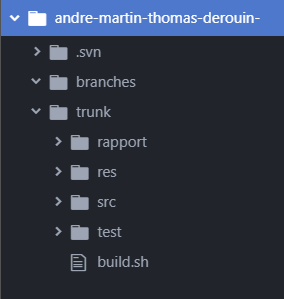
\includegraphics[width=0.5\textwidth, keepaspectratio]{img/racine.png}
		\end{figure}

		On y retrouve 4 dossiers et 1 fichier:

		\begin{itemize}
			\item le dossier \textit{rapport}, contenant ce rapport sous latex
			\item le dossier \textit{res}, conteant les ressources du jeu, ce qui correspond à l’image par défaut pour le taquin
			\item le dossier \textit{src} contenant le code source de l’application
			\item le dossier \textit{test} contenant le code se chargeant des tests unitaires
			\item le fichier \textit{build.sh}, qui permet l’execution de l’application.
		\end{itemize}

		Le code source du projet est situé dans le chemin \textit{src/taquin/}. Il est constitué par :

		\begin{figure}[H]
			\centering
			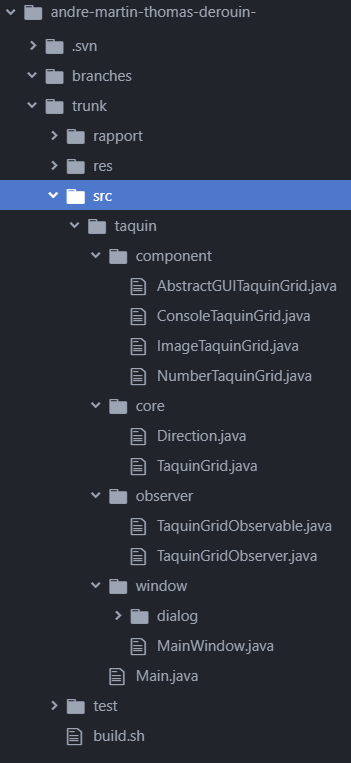
\includegraphics[width=0.5\textwidth, keepaspectratio]{img/detail.png}
		\end{figure}

		\begin{itemize}
			\item un package \textit{component}, contenant les classes des différents modes qui composent l’application.
			\item un package  \textit{core} contenant le cœur du jeu du taquin, qui est commun à tout les modes de jeu, ainsi que la classe qui énumère les directions
			\item un package \textit{observer} qui constitue le pattern Observer
			\item un package \textit{window} contenant les classes permettant de gérer ce qui se rapporte à la fenêtre de jeu et des boites de dialogues
			\item un fichier \textit{Main.java}, qui est le fichier executable du taquin
		\end{itemize}

	\section{Mise en place du pattern M-VC}

	Dans notre application, le pattern M-VC à été mis en place de la manière suivante:

	\begin{figure}[H]
		\centering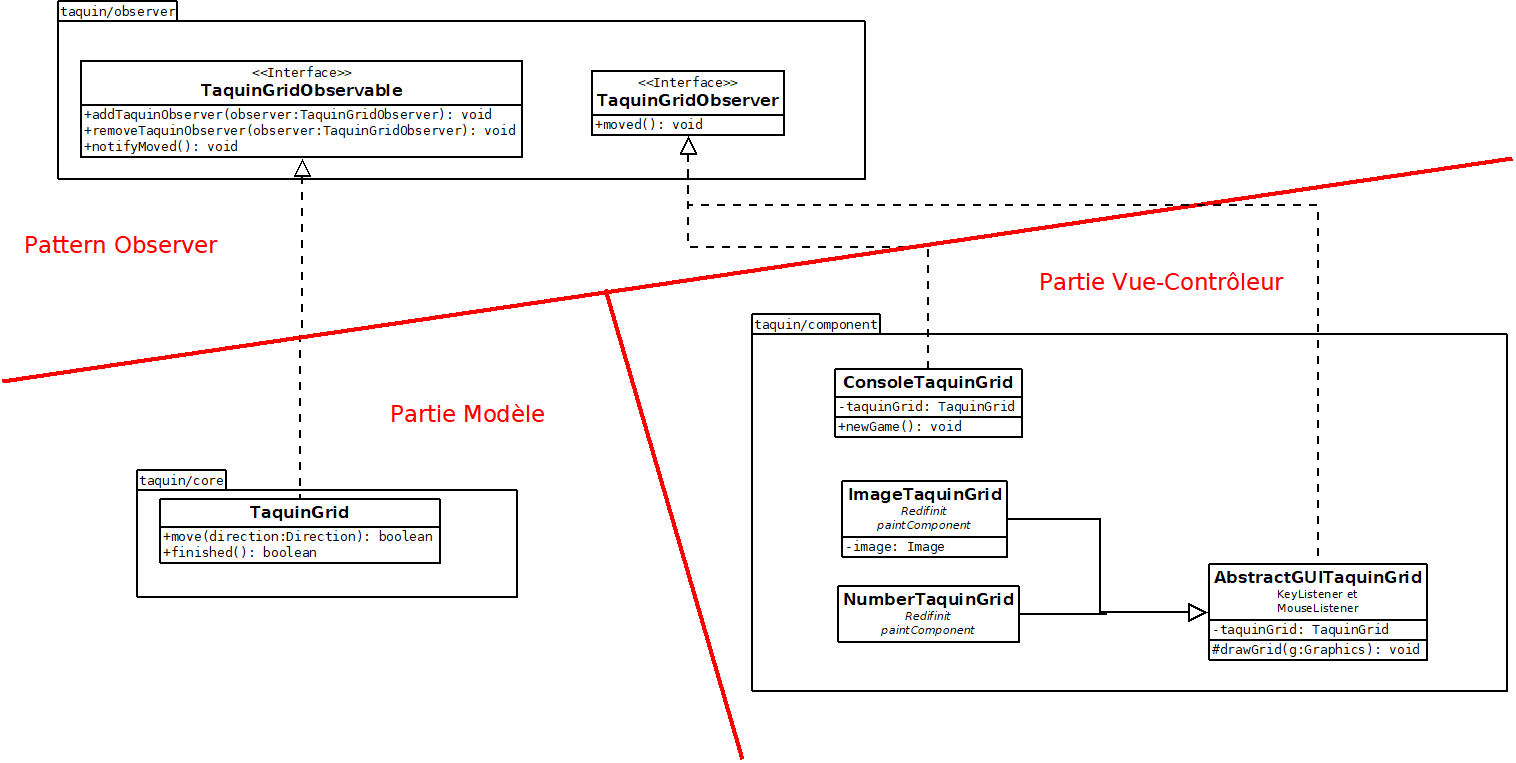
\includegraphics[width=1\textwidth, keepaspectratio]{img/diagramMVC.png}
		\caption{Notre tableau Trello}
		\label{Mise en place du M-VC}
	\end{figure}

	On a d'une part la classe \textit{TaquinGrid} représente le modèle de l'application. Il s'agit du coeur du jeu, du fonctionnement du taquin, peut importe le mode d'affichage du jeu.

	D'un autre côté, nous avons tout le package compoment, qui lui, contient les différentes vues de l'application. On retrouve dans le taquin trois vues:

	\begin{itemize}
		\item le mode "console", représenté par la classe \textit{ConsoleTaquinGrid}
		\item le mode "image", représenté par la classe \textit{ImageTaquinGrid}
		\item enfin, le mode "nombre" représenté par la classe \textit{NumberTaquinGrid}
	\end{itemize}

	La classe \textit{AbstractGUITaquinGrid} est uniquement une vue qui regroupe les parties communes aux classes \textit{ImageTaquinGrid} et \textit{NumberTaquinGrid}.

	Ces trois classes citées ci-dessus sont également des contrôleurs puisqu'elles ....
